\section{Flux-limiters}
\label{sec:fld_vef_factors}

Levermore et. al~\cite{Levermore81} construct their theory by starting from the time-dependent form of the radiative transfer equation. They further assume a constant phase function $f_p=1/(4\pi)$:
\begin{align}
\label{eq:iso_var_fld_rte}
\frac{1}{c}\frac{\partial (\phi\hat{L})}{\partial t} + \left(\vec{\omega}\cdot\nabla\right)(\phi\hat{L})&=-\sigma_t\phi\hat{L} + \frac{1}{4\pi}\sigma_s\phi + Q
\end{align}
After applying the moment expansion, for the first moment equations are as follows:
\begin{align}
\label{eq:iso_var_fld_rte_zero}
\frac{1}{c}\frac{\partial \phi}{\partial t} + \nabla\vec{E} &= -\sigma_a\phi + Q_0
\end{align}
As a next step, equation~\ref{eq:iso_var_fld_rte_zero} is resolved for $\partial \phi/\partial t$ on the left hand side and used to substitute $\partial\phi/\partial t$ in equation~\ref{eq:iso_var_fld_rte} (after applying the product rule to the time derivative term). By further assuming the absence of self-emission ($Q=0$) and that the space and time derivatives of the radiance distribution $\hat{L}$ can be neglected, the result is:
\begin{align}
\label{eq:iso_var_fld_eliminated_time}
\left( \left(\vec{\omega}\cdot\nabla\right)\phi -\vec{f}\cdot\nabla\phi + \sigma_t'\phi\right)\hat{L} = \frac{1}{4\pi}\sigma_t'\phi
\end{align}
Solving equation~\ref{eq:iso_var_fld_eliminated_time} for $\hat{L}$ gives:
\begin{align}
\label{eq:iso_var_fld_Lhat}
\hat{L} = \frac{1}{4\pi}\frac{1}{1+\widehat{\vec{E}}\cdot\vec{R}-\vec{\omega}\cdot\vec{R}}
\end{align}
with
\begin{align}
\label{eq:iso_var_fld_R}
\vec{R} = -\frac{\nabla\phi}{\sigma_t'\phi}
\end{align}
The definition of the flux-vector in equation~\ref{eq:second_moment_iso3} is used, which was derived in section~\ref{sec:fld_streaming_limit_approximation}:
\begin{align}
\widehat{\vec{E}} = \frac{\vec{E}}{\phi}= T\vec{R}
\label{eq:iso_var_fld_normalized_flux}
\end{align}

Following the same argument about the radial symmetry of $\hat{L}$ and its relation to the flux-vector and eigenvectors of $T$, $T$ is replaced with a proportionality function $\lambda(R)$, where $R=\norm{\vec{R}}$:
\begin{align}
\widehat{\vec{E}} = \lambda(R)\vec{R}
\label{eq:iso_var_fld_relation_normalized_flux_R}
\end{align}

Using this in equation~\ref{eq:iso_var_fld_Lhat} gives:
\begin{align}
\label{eq:iso_var_fld_Lhat_R}
\hat{L} = \frac{1}{4\pi}\frac{1}{1+\lambda(R)R^2-\vec{\omega}\cdot\vec{R}}
\end{align}

By enforcing that $\hat{L}$ integrates to one over the solid angle of the unit sphere, the following expression for $\lambda(R)$ can be derived:
\begin{align}
\label{eq:iso_var_fld_lambdaR}
\lambda(R) = \frac{1}{R}\left(\mathbf{\operatorname{coth}}R - \frac{1}{R}\right)
\end{align}

Using this result and equation~\ref{eq:iso_var_fld_relation_normalized_flux_R}, gives the following expression for the flux vector:
\begin{align}
\label{eq:iso_var_fld_fluxvector}
\vec{E} = \widehat{\vec{E}}\phi=-\frac{1}{\sigma_t'}\lambda(R)\nabla\phi
\end{align}

Inserting this into the zero moment equation (equation~\ref{eq:me_zero}) gives the flux-limited diffusion equation, a diffusion-type equation of the following form:
\begin{align}
\label{eq:iso_var_fld_final}
\nabla\left( \underbrace{-\frac{1}{\sigma_t'}\lambda(R)}_{D_F}\nabla\phi\right) &= -\sigma_a\phi + Q_0
\end{align}

The flux-limited diffusion coefficient $D_F$ is non-linear and therefore turns the zero moment equation into a non-linear diffusion equation. $\lambda(R)$ is called the flux-limiter. In the diffusion limit, $R$ approaches zero and the flux-limiter approaches $\lambda(R)=1/3$, which will turn equation~\ref{eq:iso_var_fld_final} into the classical diffusion equation for isotropic media.
\begin{align}
\lim_{R\rightarrow 0 }D_F =-\frac{1}{3\sigma_t'}
\implies
\nabla
\left(
-\frac{1}{3\sigma_t'\left(\vec{x}\right)}
\nabla \phi\left(\vec{x}\right)
\right)
=
-\phi(\vec{x})\sigma_a(\vec{x})
+Q_0\left(\vec{x}\right)
\end{align}
In the transport limit, $R$ will approach infinity and the diffusion coefficient will cause the equation to become an advection equation as seen in the delta radiance distribution case (equation~\ref{eq:iso_delta_advection_equation}):
\begin{align}
\lim_{R\rightarrow\infty }D_F =-\frac{\phi}{\norm{\nabla\phi}}
\implies
\nabla
\left(
-\phi\frac{\nabla\phi\left(\vec{x}\right)}{\norm{\nabla\phi}}
\right)
=
-\phi(\vec{x})\sigma_a(\vec{x})
+Q_0\left(\vec{x}\right)
\end{align}
It can be seen that the flux-limited diffusion coefficient will normalize the fluence gradient $\nabla\phi$ to unit length and scale with the total power $\phi$. Flux-limited diffusion not only suppresses the flux in the free streaming transport regime, it also saturates it at the appropriate value to ensure correct free propagation (at the level of the approximation).

The flux-limiter introduced by Levermore et al.~\cite{Levermore81} was shown to relate to the variable Eddington factor approach in a seperate study (\cite{Whalen82, Levermore84}) to be:
\begin{align}
\label{eq:iso_var_fld_vef}
\chi = \lambda(R) + \lambda(R)^2R^2
\end{align}
As mentioned in the previous section, the theory sets up the limits, which flux-limiters have to respect. This allows different models and theories to find and justify particular choices of flux-limiters. Table~\ref{tbl:flux-limiters} presents the most prominent flux-limiters.
\begin{table}[h]
\center
\caption{Various prominent flux-limiters which all respect the Eddington factor limits and represent different flux-limited diffusion theories.}
\begin{tabular}{ l l }
\hline\hline
 Flux-limiter & $\lambda\left(R\right)$ \\ 
\hline
 sum~\cite{Bowers82} & $(3+R)^{-1}$ \\
 max~\cite{Bowers82} & $\mbox{max}(3, R)^{-1}$ \\
 Kershaw~\cite{Kershaw76} & $2(3+\sqrt{9 + 4R^2}\,)^{-1}$ \\
 Larsen-$n$~\cite{Larsen74} & $(3^n + R^n)^{-\frac{1}{n}}$ \\
 Levermore-Pomraning~\cite{Levermore81} & $\frac{1}{R} \left(\coth(R)-\frac{1}{R}\right)$    
\end{tabular}
\label{tbl:flux-limiters}
\end{table}

\begin{figure}[h]
\centering
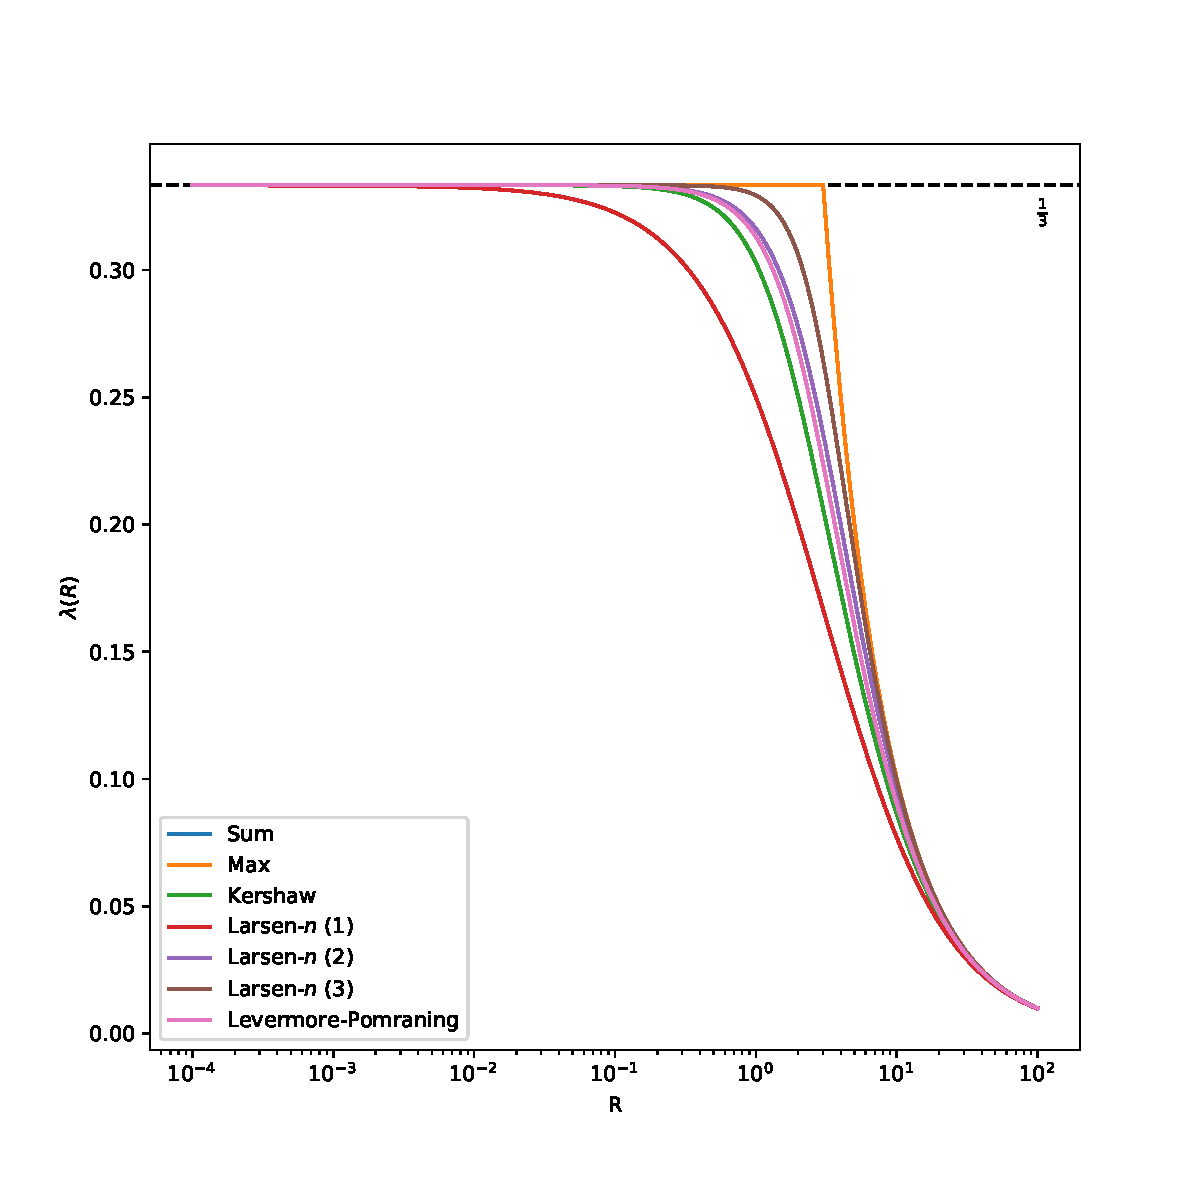
\includegraphics[width=0.65\textwidth]{06_fld/figures/plot_flux_limiters.pdf}
\caption{Plot of the various flux-limiters shown in table~\ref{tbl:flux-limiters}.}
\label{fig:flux-limiters}
\end{figure}
%
%\missingfigure{flux-limiters graphs}

In this section a non-linear form of the diffusion equation is derived which respects the flux-limit constraint. The following section will present a novel solver, which solves flux-limited diffusion on a finite difference grid over a given domain.